\documentclass{minimal}

\usepackage{pdflscape}
\usepackage{tikz}

\usetikzlibrary{er, positioning, fit}
\tikzset{multi attribute/.style = {attribute, double distance=1.5pt}}
\tikzset{total relation/.style = {-, double, double distance=1.5pt}}

\begin{document}

\begin{landscape}
  \begin{center}
    \resizebox{20cm}{!}{%
    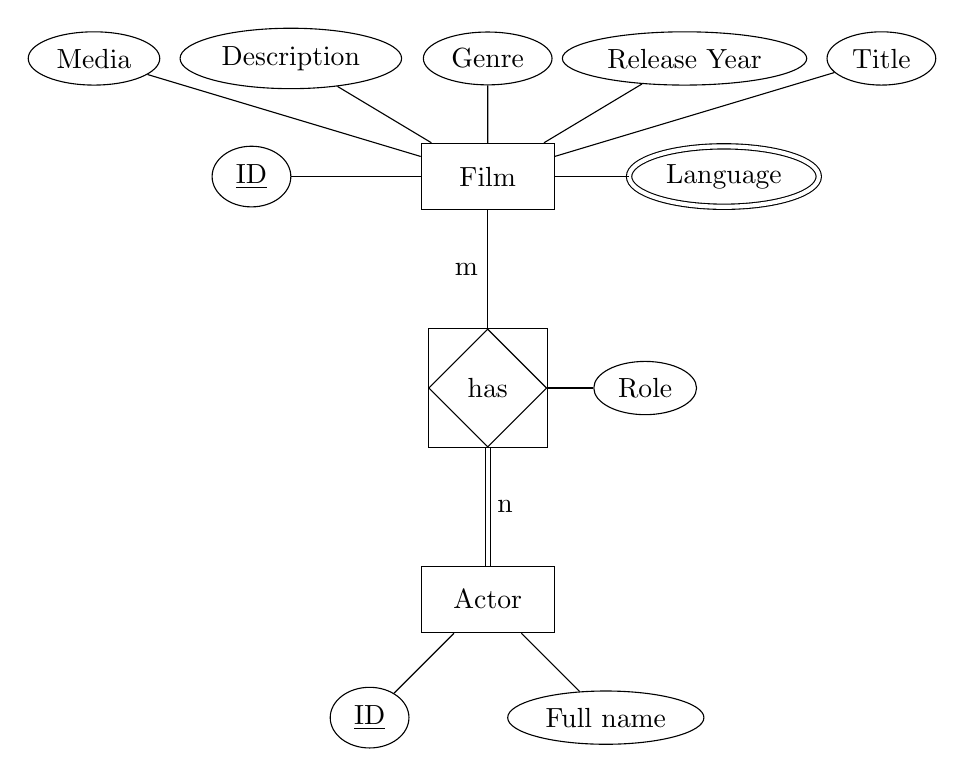
\begin{tikzpicture}[auto,node distance=1.5cm]
      \node[entity] (film) {Film}
        [grow=up,sibling distance=2.5cm]
        child[grow=left, level distance=3cm] {node[attribute, minimum width =
        1cm]
        {\underline{ID}}} 
        child {node[attribute] {Title}}
        child {node[attribute] {Release Year}}
        child {node[attribute] {Genre}}
        child {node[attribute] {Description}}
        child {node[attribute] {Media}}
        child[grow=right, level distance=3cm] {node[multi attribute] {Language}};

      \node[relationship] (relFilmActor) [below = of film, minimum size=1.5cm]
      {has}
      child[grow=right, level distance=2cm] {node[attribute] {Role}};

      \node[rectangle, draw=black, fit=(relFilmActor), inner sep=0em]
        (relFilmActorSq) {};

      \node[entity] (actor) [below = of relFilmActor] {Actor}
        [grow = down, sibling distance=3cm]
        child {node[attribute, minimum width = 1cm] {\underline{ID}}}
        child {node[attribute] {Full name}};
                        
      \path (relFilmActor)
        edge node {m} (film)
        edge[total relation] node {n} (actor);
    \end{tikzpicture}
    }
  \end{center}
\end{landscape}

\end{document}